\chapter*{Acknowledgements}

\markboth{Acknowledgements}{Acknowledgements}
\addcontentsline{toc}{chapter}{Acknowledgements}


This thesis would not have come to fruition without the help, understanding, and presence of many people, whom I will mention here.

First, I would like to thank my supervisor, Laura, who went to great lengths to help me find my way in the mathematical sciences.
I am grateful for the opportunities you have given me, the clear guidance in the first years, and the trust you placed in me when I started to branch out towards more computational research topics.
I wish I could explain to your future students how much I appreciated your supervision, so maybe you can stick this somewhere:
\begin{center}
    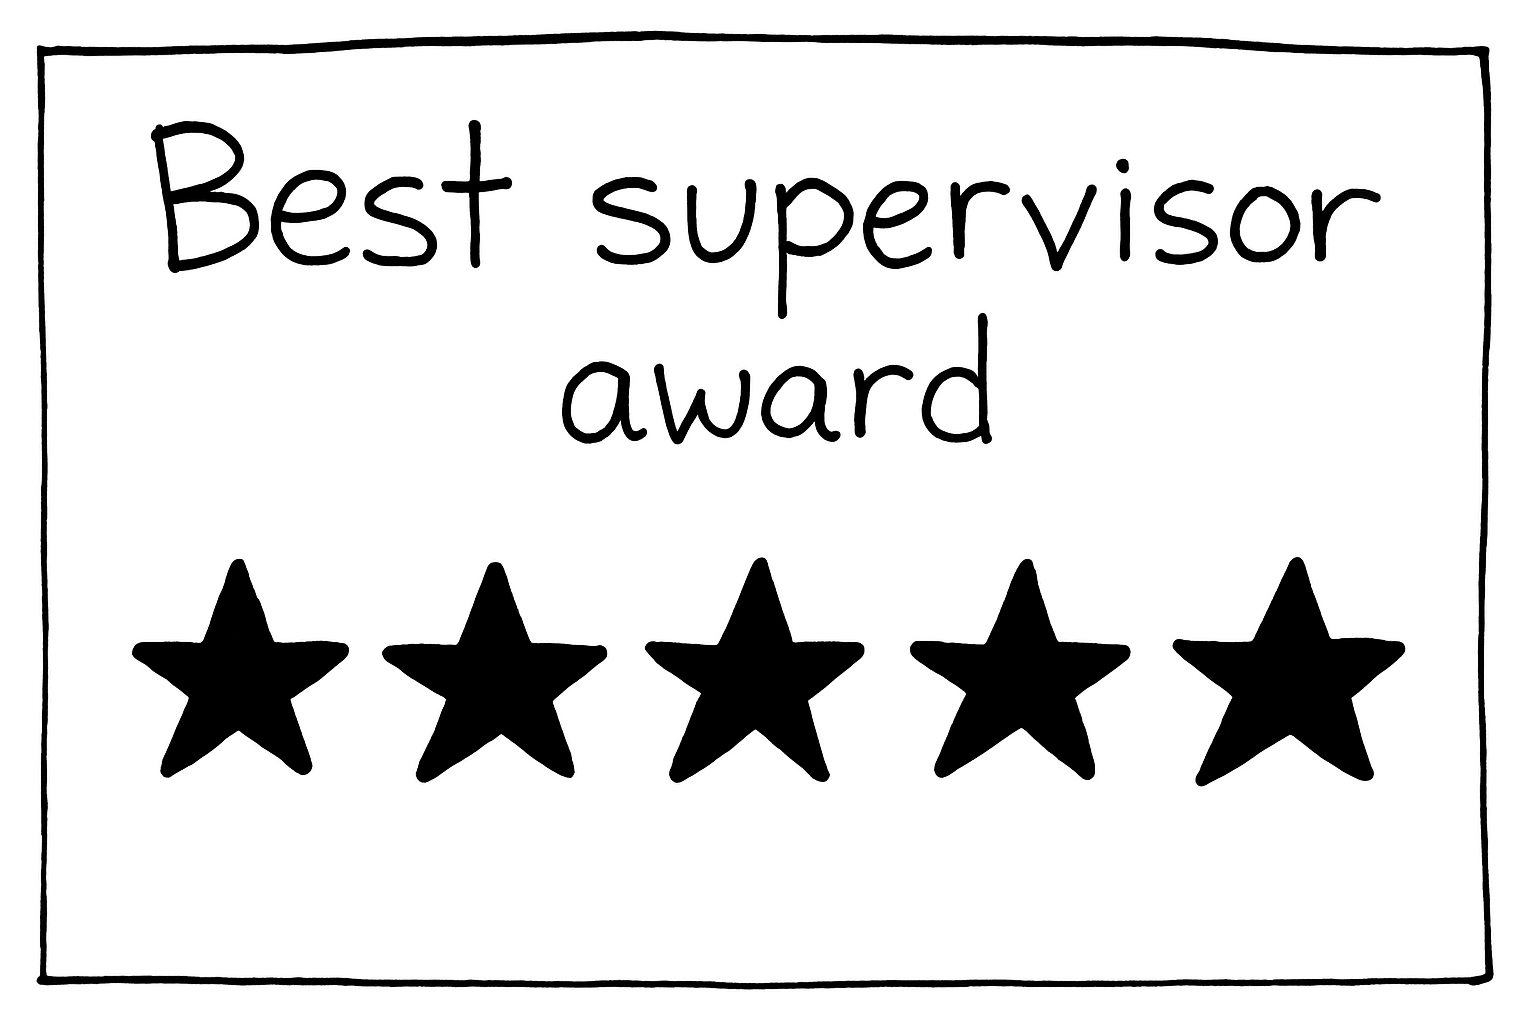
\includegraphics[width=0.45\textwidth]{award}
\end{center}
My supervision would not have been complete without my promotor, Gabriel.
Although you had limited time due to administrative duties, any opportunity to catch up, even in the hallway or on the bike, was always a positive experience.
You warned me whenever results came in (too) fast, and were happy for me when the correct results finally came rolling in.

To the members of the manuscript committee, thank you for taking the time to read, evaluate, and report on the manuscript of this thesis.

Special thanks go to Dokken and Nate from the Fenics project discourse group for helping me improve my understanding of the Dolfinx environment and suggesting improvements that went beyond my questions.
Similarly, I want to thank Mike Earnest on the math stack exchange for helping me with the proof of Lemma~\ref{lem:multinomialsum}.

My thanks also go to the wonderful people at Alliander, especially to Sander, Jordi, Ferran, Raymond, and the people of the Verbindingsteam.
Collectively, they let me experience their world of cables, distribution stations, and the mathematics we can use to fix real problems in the power distribution grid.

My time at the Radboud University would have been boring at best without all the colleagues in the mathematics department.
Special thanks go to Mostafa and Victor for introducing me to the department and group, and checking in whenever possible.
To Grégoire, Kevin, and the maggots for the experience of the 4-day marches and Kevin for the many, many chats, discussions, before, during, and after working hours about anything and everything.
Without all my current and former PhD colleagues, the atmosphere would not have been as friendly and relaxed as it has been, for which I am very grateful.

As the reader might pick up from the CV at the end of this thesis, much of my time has been spent with some amazing people at Scouting.
I want to thank Lukas and Joris for complaining about their PhD struggles to relate to and to show me how good my environment has been in the last few years.
I will not forget the (long) AOT and MWS hikes with Isis, Kip, Koen, Niels, and Martijn, which never failed to clear my mind of work issues and mathematical problems.
Not to forget, all other members of Radix Enschede who joined in our adventures to Bad Bentheim, Bad Bentheim, and\textemdash of course\textemdash Bad Bentheim.

In a similar vein, Trapperskampen has been a trustworthy source of distractions all year round.
Special thanks go to my fellow board members, Mark, Michel, Michiel, and Niels, for trusting me with the group finances (in their\ldots unique state).
I will also not forget the adventures I have had with my fellow staff members during Extreem and Scoutdoor.
Subtly sneaking some \emph{recreational mathematics} into conversations was a treat.

Any time I was back home, I could count on the support of my parents, Dick and Marja.
Together with the rest of my close family\textemdash Thom and Bakul, Florian and Sarah, and Jochem and Sterre\textemdash you always kept asking me what I was doing, forcing me to think about my work in non-mathematical terms.
This greatly improved my scientific communication skills and led to many enjoyable conversations, thank you so much.

And above all, nothing would have been even close to as enjoyable as it has been without my fiancée, Nynke.
You have been a part of almost all the events mentioned above in some way, bringing something funny, unique, or otherwise memorable.
Four years ago, we had just moved in together, and not long after, we explored where we wanted to live and how to make that happen, settling down in Gendt only a few years ago.
I cannot wait to see what the next chapters will bring us together.
